%                      Code_Saturne version 1.3
%                      ------------------------
%
%     This file is part of the Code_Saturne Kernel, element of the
%     Code_Saturne CFD tool.
%
%     Copyright (C) 1998-2007 EDF S.A., France
%
%     contact: saturne-support@edf.fr
%
%     The Code_Saturne Kernel is free software; you can redistribute it
%     and/or modify it under the terms of the GNU General Public License
%     as published by the Free Software Foundation; either version 2 of
%     the License, or (at your option) any later version.
%
%     The Code_Saturne Kernel is distributed in the hope that it will be
%     useful, but WITHOUT ANY WARRANTY; without even the implied warranty
%     of MERCHANTABILITY or FITNESS FOR A PARTICULAR PURPOSE.  See the
%     GNU General Public License for more details.
%
%     You should have received a copy of the GNU General Public License
%     along with the Code_Saturne Kernel; if not, write to the
%     Free Software Foundation, Inc.,
%     51 Franklin St, Fifth Floor,
%     Boston, MA  02110-1301  USA
%
%-----------------------------------------------------------------------
%

%%%%%%%%%%%%%%%%%%%%%%%%%%%%%%%%%%
%%%%%%%%%%%%%%%%%%%%%%%%%%%%%%%%%%
\section{Discr\'etisation}
%%%%%%%%%%%%%%%%%%%%%%%%%%%%%%%%%%
%%%%%%%%%%%%%%%%%%%%%%%%%%%%%%%%%%

La figure \ref{Base_Clsyvt_fig_facesym} pr\'esente les notations utilis\'ees \`a la face. Le
rep\`ere local est d\'efini \`a partir de la normale \`a la face et la vitesse
en $I'$ :\\
$\bullet\ \displaystyle\vect{t}
=\frac{1}{|\vect{u}_{I',\tau}|}\vect{u}_{I',\tau}$ est le
premier vecteur du rep\`ere local.\\
$\bullet\ \vect{\tilde{n}}=-\vect{n}$ est le deuxi\`eme vecteur du rep\`ere
local.\\
$\bullet\ \vect{b}=\vect{t}\wedge\vect{\tilde{n}}=\vect{n}\wedge\vect{t}$ est le
troisi\`eme vecteur du rep\`ere local.

\begin{figure}[h]
\centerline{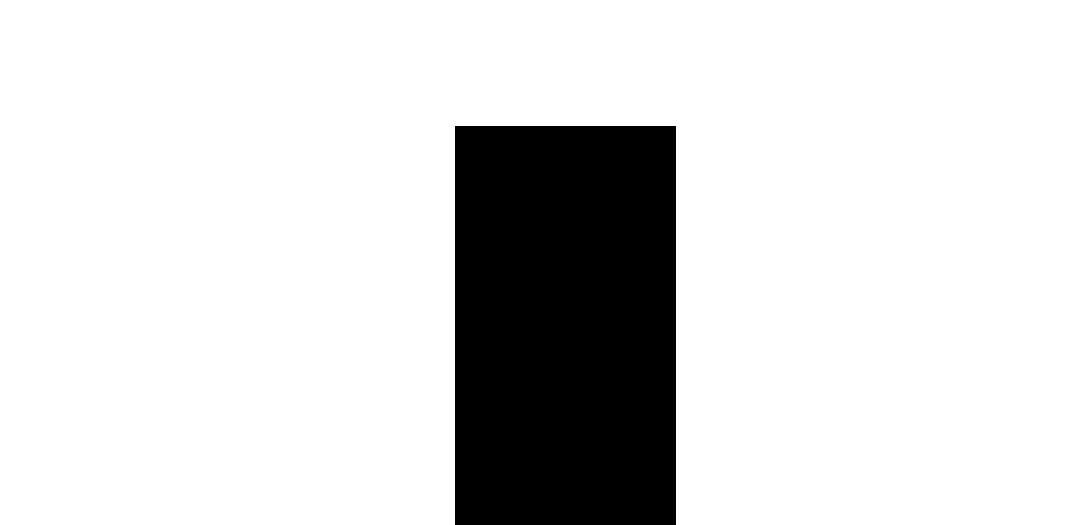
\includegraphics[width=8cm]{../Base/Clsyvt/Images/facesym.pdf}}
\caption{\label{Base_Clsyvt_fig_facesym}D\'efinition des vecteurs de base du rep\`ere local}
\end{figure}

Ici, $\vect{n}$ est la normale \`a la face de bord au sens de \CS\ ({\em i.e.}
pointant vers l'ext\'erieur) et $\vect{u}_{I',\tau}$ est la projection de la
vitesse en $I'$ dans le plan de la face :
$\vect{u}_{I',\tau}=\vect{u}_{I'}-(\vect{u}_{I'}.\vect{n})\vect{n}$.\\
Si $\vect{u}_{I',\tau}=\vect{0}$, l'orientation de $\vect{t}$ dans le plan
normal \`a $\vect{n}$ est sans importance. On le d\'efinit alors par :
$\displaystyle\vect{t}=\frac{1}{\sqrt{n_y^2+n_z^2}}(n_z\vect{e}_y-n_y\vect{e}_z)$
ou
$\displaystyle\vect{t}=\frac{1}{\sqrt{n_x^2+n_z^2}}(n_z\vect{e}_x-n_x\vect{e}_z)$
suivant les composantes de $\vect{n}$ qui sont non nulles (composantes dans le
rep\`ere global $(\vect{e}_x,\vect{e}_y,\vect{e}_z)$).


Pour plus de clart\'e, on utilisera les notations suivantes :\\
$\bullet\ $Le rep\`ere g\'en\'eral sera not\'e
$\mathcal{R}=(\vect{e}_x,\vect{e}_y,\vect{e}_z)$.\\
$\bullet\ $Le rep\`ere local sera not\'e
$\hat{\mathcal{R}}=(\vect{t},-\vect{n},\vect{b})=(\vect{t},\vect{\tilde{n}},\vect{b})$.\\
$\bullet\ $Les matrices des composantes d'un vecteur $\vect{u}$ dans les rep\`eres
$\mathcal{R}$ et $\hat{\mathcal{R}}$ seront not\'ees respectivement
$\mat{U}$ et $\hat{\mat{U}}$.\\
$\bullet\ $Les matrices des composantes d'un tenseur $\tens{R}$ (d'ordre 2) dans
les rep\`eres $\mathcal{R}$ et $\hat{\mathcal{R}}$ seront not\'ees
respectivement $\matt{R}$ et $\hat{\matt{R}}$.\\
$\bullet\ $On note $\matt{P}$ la matrice (orthogonale) de passage de $\mathcal{R}$ \`a
$\hat{\mathcal{R}}$.
\begin{equation}
\matt{P}=\left[
\begin{array}{ccc}
t_x & -n_x & b_x\\
t_y & -n_y & b_y\\
t_z & -n_z & b_z
\end{array}\right]
\end{equation}

($\matt{P}$ \'etant orthogonale, $\matt{P}^{-1}=\,^t\matt{P}$).

On a alors en particulier les relations suivantes, pour tout vecteur $\vect{u}$
et tout tenseur $\tens{R}$ d'ordre 2 :\\
\begin{equation}
\left\{\begin{array}{l}
\mat{U} = \matt{P}\,.\,\hat{\mat{U}}\\
\matt{R}= \matt{P}\,.\,\hat{\matt{R}}\,.\,^t\matt{P}
\end{array}\right.
\end{equation}

\minititre{Traitement de la vitesse}
Dans le rep\`ere local, les conditions aux limites pour $\vect{u}$ s'\'ecrivent
naturellement :\\
\begin{equation}
\left\{\begin{array}{lcl}
u_{F,t} & = & u_{I',t}\\
u_{F,\tilde{n}} & = & 0\\
u_{F,b} & = & u_{I',b}
\end{array}\right.
\end{equation}

Soit
\begin{equation}
\mat{U}_F = \matt{P}\,.\,\hat{\mat{U}}_F
= \matt{P}\,.\,\left[
\begin{array}{ccc}
1 & 0 & 0\\
0 & 0 & 0\\
0 & 0 & 1
\end{array}
\right]\,.\,\hat{\mat{U}}_{I'}
=\matt{P}\,.\,\left[
\begin{array}{ccc}
1 & 0 & 0\\
0 & 0 & 0\\
0 & 0 & 1
\end{array}
\right]\,.\,^t\matt{P}\,.\,\mat{U}_{I'}
\end{equation}


On pose
$\matt{A}=\matt{P}\,.\,\left[
\begin{array}{ccc}
1 & 0 & 0\\
0 & 0 & 0\\
0 & 0 & 1
\end{array}
\right]\,.\,^t\matt{P}\qquad$ (matrice dans le rep\`ere $\mathcal{R}$ du projecteur
orthogonal \`a la face).

Les conditions aux limites pour $\vect{u}$ s'\'ecrivent donc :
\begin{equation}
\mat{U}_F = \matt{A}\,.\,\mat{U}_{I'}
\end{equation}

La matrice $\matt{P}$ \'etant orthogonale, on montre que
\begin{equation}
\matt{A}=\left[
\begin{array}{ccc}
1-\tilde{n}_x^2 & -\tilde{n}_x\tilde{n}_y & -\tilde{n}_x\tilde{n}_z\\
-\tilde{n}_x\tilde{n}_y & 1-\tilde{n}_y^2 & -\tilde{n}_y\tilde{n}_z\\
-\tilde{n}_x\tilde{n}_z & -\tilde{n}_y\tilde{n}_z & 1-\tilde{n}_z^2
\end{array}\right]
\end{equation}

Les conditions aux limites peuvent alors \^etre implicit\'ees partiellement, en
\'ecrivant :
\begin{equation}
\label{Base_Clsyvt_eq_clU}
u_{F,x}^{(n+1)} = \underbrace{1-\tilde{n}_x^2}_{\var{COEFB}}u_{I',x}^{(n+1)}
\underbrace{-\tilde{n}_x\tilde{n}_y u_{I',y}^{(n)}
-\tilde{n}_x\tilde{n}_z u_{I',z}^{(n)}}_{\var{COEFA}}
\end{equation}

Le traitement des deux autres composantes est similaire. On note que seules les
coordonn\'ees de $\vect{n}$ sont utiles, il n'est donc pas n\'ecessaire (pour
$\vect{u}$) de d\'efinir concr\`etement les vecteurs $\vect{t}$ et $\vect{b}$.

\vspace{1cm}
\minititre{Traitement du tenseur de Reynolds}
On a vu qu'on avait la relation suivante :
\begin{equation}
\label{Base_Clsyvt_eq_chgtrepR}
\matt{R}= \matt{P}\,.\,\hat{\matt{R}}\,.\,^t\matt{P}
\end{equation}

Les conditions aux limites que l'on cherche \`a \'ecrire sont des relations du
type :
\begin{equation}
\comp{R}_{F,ij}=\sum_{k,l}\alpha_{ijkl}\comp{R}_{I',kl}
\end{equation}
On est donc amen\'e assez naturellement \`a introduire les matrices colonne des
composantes de $\tens{R}$ dans les diff\'erents rep\`eres.

On pose
\begin{equation}
\mat{S}=\,^t[\comp{R}_{11},\comp{R}_{12},\comp{R}_{13},
\comp{R}_{21},\comp{R}_{22},\comp{R}_{23},
\comp{R}_{31},\comp{R}_{32},\comp{R}_{33}]
\end{equation}
et
\begin{equation}
\hat{\mat{S}}=\,^t[\hat{\comp{R}}_{11},\hat{\comp{R}}_{12},\hat{\comp{R}}_{13},
\hat{\comp{R}}_{21},\hat{\comp{R}}_{22},\hat{\comp{R}}_{23},
\hat{\comp{R}}_{31},\hat{\comp{R}}_{32},\hat{\comp{R}}_{33}]
\end{equation}

On introduit deux applications $q$ et $r$ de $\{1,2,3,4,5,6,7,8,9\}$ dans
$\{1,2,3\}$ dont les valeurs sont donn\'ees dans le tableau suivant :
\begin{center}
\begin{tabular}{|c|c|c|c|c|c|c|c|c|c|}
\hline
$i$&1&2&3&4&5&6&7&8&9\\
\hline
$q(i)$&1&1&1&2&2&2&3&3&3\\
\hline
$r(i)$&1&2&3&1&2&3&1&2&3\\
\hline
\end{tabular}
\end{center}
$i\longmapsto (q(i),r(i))$ est alors une bijection de $\{1,2,3,4,5,6,7,8,9\}$
dans $\{1,2,3\}^2$, et on a :
\begin{equation}
\left\{\begin{array}{l}
\comp{R}_{ij}=\comp{S}_{3(i-1)+j}\\
\comp{S}_i=\comp{R}_{q(i)r(i)}
\end{array}\right.
\end{equation}

D'apr\`es l'\'equation \ref{Base_Clsyvt_eq_chgtrepR}, on a donc :
\begin{eqnarray}
\comp{S}_{F,i} & = & \comp{R}_{F,q(i)r(i)} =
\sum_{(m,n)\in\{1,2,3\}^2}\comp{P}_{q(i)m}\hat{\comp{R}}_{F,mn}\comp{P}_{r(i)n}\nonumber\\
&=&\sum_{j=1}^9\comp{P}_{q(i)q(j)}\hat{\comp{R}}_{F,q(j)r(j)}\comp{P}_{r(i)r(j)}
\quad\text{(d'apr\`es la bijectivit\'e de $(q,r)$)}\nonumber\\
&=&\sum_{j=1}^9\comp{P}_{q(i)q(j)}\comp{P}_{r(i)r(j)}\hat{\comp{S}}_{F,j}
\end{eqnarray}

Soit
\begin{equation}
\mat{S}_{F}=\matt{A}\,.\,\hat{\mat{S}}_F\quad\text{avec }
\comp{A}_{ij}=\comp{P}_{q(i)q(j)}\comp{P}_{r(i)r(j)}
\end{equation}

On peut montrer que $\matt{A}$ est une matrice orthogonale (cf. Annexe A).

Dans le rep\`ere local, les conditions aux limites de $\tens{R}$ s'\'ecrivent de
mani\`ere naturelle\footnote{cf. Davroux A., Archambeau F., {\em Le
$R_{ij}-\varepsilon$ dans \CS\ (version $\beta$)}, HI-83/00/030/A}.
\begin{equation}
\label{Base_Clsyvt_eq_clRij}%
\left\{\begin{array}{lll}
\hat{\comp{R}}_{F,11}=\hat{\comp{R}}_{I',11} \qquad\qquad&
\hat{\comp{R}}_{F,21}=0 \qquad\qquad&
\hat{\comp{R}}_{F,31}=B\hat{\comp{R}}_{I',31} \\
\hat{\comp{R}}_{F,12}=0 \qquad\qquad&
\hat{\comp{R}}_{F,22}=\hat{\comp{R}}_{I',22} \qquad\qquad&
\hat{\comp{R}}_{F,32}=0 \\
\hat{\comp{R}}_{F,13}=B\hat{\comp{R}}_{I',13} \qquad\qquad&
\hat{\comp{R}}_{F,23}=0 \qquad\qquad&
\hat{\comp{R}}_{F,33}=\hat{\comp{R}}_{I',33}
\end{array}\right.
\end{equation}

soit
\renewcommand{\arraystretch}{0.5}
\begin{equation}
\hat{\mat{S}}_F=\matt{B}\,.\,\hat{\mat{S}}_{I'}
\qquad\text{avec }\matt{B}=
\left[\begin{array}{ccccccccc}
1&0&\cdots&\cdots&\cdots&\cdots&\cdots&\cdots&0\\
0&0&\ddots&&&&&&\vdots\\
\vdots&\ddots&B&\ddots&&&&&\vdots\\
\vdots&&\ddots&0&\ddots&&&&\vdots\\
\vdots&&&\ddots&1&\ddots&&&\vdots\\
\vdots&&&&\ddots&0&\ddots&&\vdots\\
\vdots&&&&&\ddots&B&\ddots&\vdots\\
\vdots&&&&&&\ddots&0&0\\
0&\cdots&\cdots&\cdots&\cdots&\cdots&\cdots&0&1
\end{array}\right]
\end{equation}
\renewcommand{\arraystretch}{1.}

Dans le cas des faces de sym\'etries trait\'ees par \fort{clsyvt}, le
coefficient $B$ vaut 1. Mais un traitement similaire est r\'ealis\'e dans
\fort{clptur} pour les faces de paroi, et dans ce cas $B$ est nul. Ce
param\`etre devra \^etre sp\'ecifi\'e dans l'appel \`a \fort{clca66}
(cf. \S\ref{Base_Clsyvt_prg_meo}).

En retournant dans le rep\`ere global, on obtient finalement la formule suivante
:
\begin{equation}
\label{Base_Clsyvt_eq_clsurS}
\mat{S}_F=\matt{C}\,.\,\mat{S}_{I'}\qquad
\text{avec }\matt{C}=\matt{A}\,.\,\matt{B}\,.\,^t\matt{A}
\end{equation}

On peut montrer que la matrice $\matt{C}$ a pour composantes :
\begin{equation}
\comp{C}_{ij}=\sum_{k=1}^9
\comp{P}_{q(i)q(k)}\comp{P}_{r(i)r(k)}\comp{P}_{q(j)q(k)}\comp{P}_{r(j)r(k)}
(\delta_{k1}+B\delta_{k3}+\delta_{k5}+B\delta_{k7}+\delta_{k9})
\end{equation}


Pour finir, on note que la matrice $\mat{S}$ est redondante, du fait des
sym\'etries du tenseur $\tens{R}$. On va donc plus simplement utiliser les
matrices r\'eduites $\mat{S}^\prime$ et $\hat{\mat{S}}^\prime$ :
\begin{equation}
\mat{S}^\prime=\,^t[\comp{R}_{11},\comp{R}_{22},\comp{R}_{33},
\comp{R}_{12},\comp{R}_{13},\comp{R}_{23}]
\end{equation}
\begin{equation}
\hat{\mat{S}}^\prime=\,^t[\hat{\comp{R}}_{11},\hat{\comp{R}}_{22},\hat{\comp{R}}_{33},
\hat{\comp{R}}_{12},\hat{\comp{R}}_{13},\hat{\comp{R}}_{23}]
\end{equation}

En regroupant diff\'erentes lignes de la matrice $\matt{C}$, on transforme
l'\'equation \ref{Base_Clsyvt_eq_clsurS} en l'\'equation finale suivante :
\begin{equation}
\mat{S}_F^\prime=\matt{D}\,.\,\mat{S}_{I'}^\prime
\end{equation}

Le calcul de la matrice $\matt{D}$ est r\'ealis\'e dans le sous-programme
\fort{clca66}. La m\'ethodologie est d\'ecrite en annexe B.

\`A partir de $\matt{D}$, on peut exprimer les coefficients des conditions aux
limites, partiellement implicites ($\var{ICLSYR}=1$) ou totalement explicites
($\var{ICLSYR}=0$).

$\bullet\ ${\sc Implicitation partielle}\\
\begin{equation}
\label{Base_Clsyvt_eq_clRimp}
{\comp{S}_{F,i}^\prime}^{(n+1)} =
\underbrace{\comp{D}_{ii}}_{\var{COEFB}}{\comp{S}_{I',i}^\prime}^{(n+1)}
+\underbrace{\sum_{j\ne i}\comp{D}_{ij}{\comp{S}_{I',j}^\prime}^{(n)}}_{\var{COEFA}}
\end{equation}

$\bullet\ ${\sc Explicitation totale}\\
\begin{equation}
\label{Base_Clsyvt_eq_clRexp}
{\comp{S}_{F,i}^\prime}^{(n+1)} =
\underbrace{\sum_j\comp{D}_{ij}{\comp{S}_{I',j}^\prime}^{(n)}}_{\var{COEFA}}
\qquad(\var{COEFB}=0)
\end{equation}
